\documentclass[11pt,a4paper]{article}
\usepackage{fontspec}
\setmainfont{TeX Gyre Pagella}
\newfontfamily\headfont{Inter}[UprightFont=*-ExtraBold,BoldFont=*-ExtraBold,Extension=.otf,Path=/usr/share/fonts/opentype/inter/]
\usepackage[a4paper,margin=2.3cm]{geometry}
\usepackage{graphicx,booktabs,float,caption,array,xcolor,longtable}
\usepackage{xurl}
\usepackage[hidelinks]{hyperref}
\usepackage{titlesec}
\usepackage[round]{natbib}
\usepackage{setspace}
\setstretch{1.05}
\renewcommand{\topfraction}{0.9}
\renewcommand{\bottomfraction}{0.8}
\renewcommand{\textfraction}{0.1}
\renewcommand{\floatpagefraction}{0.75}
\setlength{\parindent}{0pt}
\setlength{\parskip}{0.55em}
\titleformat{\section}{\headfont\Large}{\thesection}{0.8em}{}
\titleformat{\subsection}{\headfont\large}{\thesubsection}{0.8em}{}
\captionsetup{font=small,labelfont=bf}
\urlstyle{same}
\hypersetup{pdftitle={HMS Your Town},pdfauthor={Tristan Hotham}}

\begin{document}
\begin{center}
{\Large\bfseries HMS Your Town\par}
\vspace{0.4em}
{\large British towns and the Royal Navy ships named after them, from Wikidata\par}
\vspace{1.2em}
{\large Tristan Hotham\par}
\vspace{0.3em}
{\small Independent researcher\\
ORCID: 0000-0003-4931-9349\\
DOI: https://doi.org/10.5281/zenodo.24052719\par}
\vspace{0.8em}
2026
\end{center}

\begin{quote}
\small
\begin{center}\textbf{Abstract}\end{center}
Many British towns have given their name to a warship. I ask which towns, how often, when, and what became of the ships, using the 6,006 Royal Navy ships named ``HMS'' in Wikidata. Because Wikidata records what a ship was named after for only 261 of them, I match ship names strictly to British towns and cities, excluding classes and names that honour other things, and flag names that are also noble titles. The result is 394 ships named after 135 towns and cities. Gloucester and Newcastle upon Tyne have had nine ships each; 28 towns have had five or more and 50 just one. 63\% of the towns lie within 10 km of the open sea. Town names were common in the later 1600s (33\% of ships commissioned 1650 to 1699), rare through the 1800s (under 3\%) and common again after 1950 (23\%). The question of fate can hardly be answered from open data: only 24\% of the ships have any recorded end, 11 of them a loss. Ships named after places in other navies' Wikidata records show the same habit, most of all in the United States Navy (146 ships named after American towns and cities).

\textbf{Keywords:} naval history; ship names; Royal Navy; toponymy; Wikidata; civic identity; open data
\end{quote}

\section{Introduction}
A warship named after a town is a link between the town and the Navy: the ship carries the town's name, crest and often gifts from its people, and the town follows the ship. This short study asks which British towns have been honoured in this way, how many times, in which eras, and what happened to the ships. It accompanies an interactive map (\url{https://maps.tristanhotham.com/ships-named/}).

\section{Data}
\textbf{Ships.} The ships are the items in Wikidata \citep{wikidata} operated by the Royal Navy whose label begins ``HMS'' (6,006 ships), with their class, commissioning and decommissioning dates where present, their significant events (launch, commissioning, sinking, shipwreck, breaking up and so on) and, for 261 ships, the item they are named after (property P138). A second extract lists ships of all navies with P138 pointing to a place with coordinates, used for the international comparison.

\textbf{Towns.} British towns and cities come from Wikidata's settlements in the United Kingdom, with coordinates, population and type. For matching I keep places typed as town, market town, city, county town, seaside resort or new town, or with 10,000 people or more, inside the bounds of the United Kingdom.

\section{Methods}
\subsection{Matching ships to towns}
A ship is linked to a town in one of three ways. Where its P138 is a British town or city, that town is used (10 ships). Otherwise its name after ``HMS'' must equal a town's name exactly (350 ships), or be ``\textit{town} Castle'', for ships named after a town's castle (34 ships, most of them Castle-class corvettes of 1944). Where several towns share a name, the most populous is used and the match flagged; common short forms are mapped to the town the Navy meant (Newcastle to Newcastle upon Tyne, Yarmouth to Great Yarmouth, Berwick to Berwick-upon-Tweed, Londonderry to Derry, Shoreham to Shoreham-by-Sea, Milford to Milford Haven, Weston to Weston-super-Mare), and three castles are placed where they stand (Leeds Castle, in Kent, is excluded; Caistor Castle is Caister Castle in Norfolk; Hadleigh Castle is in Essex). Excluded are ships whose P138 is anything but a British town (a person, a foreign place, a county or a river), classes named after other things (the Hunt-class destroyers after fox hunts, the Racecourse-class after racecourses, the River, Flower, Bird, Tree, Isles and Dance classes, and the classes named after counties: the Monmouth and Devonshire armoured cruisers, the County-class heavy cruisers and the County-class destroyers), and a list of names that honour people, battles, rivers, counties or foreign places though a British town shares them (Nelson, Wellington, Marlborough, Dunkirk, Gibraltar, Halifax, Colne and others; the list is in the code). In all 675 ships were excluded by these rules. Names that are also titles of royal dukes or peers (York, Gloucester, Lancaster, Newcastle and others) are kept but flagged: 167 ships carry such a name, and some of the older ones may honour the duke or earl rather than the town.

\subsection{Years and fates}
A ship's year is its commissioning year (266 matched ships); otherwise the median commissioning year of its class when three or more members are dated, or the year in the name of an ``Establishment'' class (54 ships). 320 of the 394 ships have a year. Fates come from the ship's events, in this order of precedence: sunk, wrecked, scuttled or destroyed; captured; broken up or scrapped; sold or transferred; decommissioned; and, for ships commissioned since 1985 with no end recorded, ``in service or recent''.

\section{Results}
\subsection{Which towns}
Figure~\ref{fig:map} maps the 135 towns. 112 are in England, 12 in Scotland, 8 in Wales and 3 in Northern Ireland. The most-named (Figure~\ref{fig:top}) are Gloucester and Newcastle upon Tyne with nine ships each, Glasgow with eight, and Chatham, Falmouth, London, Maidstone, Pembroke, Scarborough and York with seven. They are old ports, cathedral cities and the dockyard towns of the Navy. 85 of the towns (63\%) lie within 10 km of the open sea, measured to the Natural Earth coastline \citep{naturalearth}.

\begin{figure}[tbp]\centering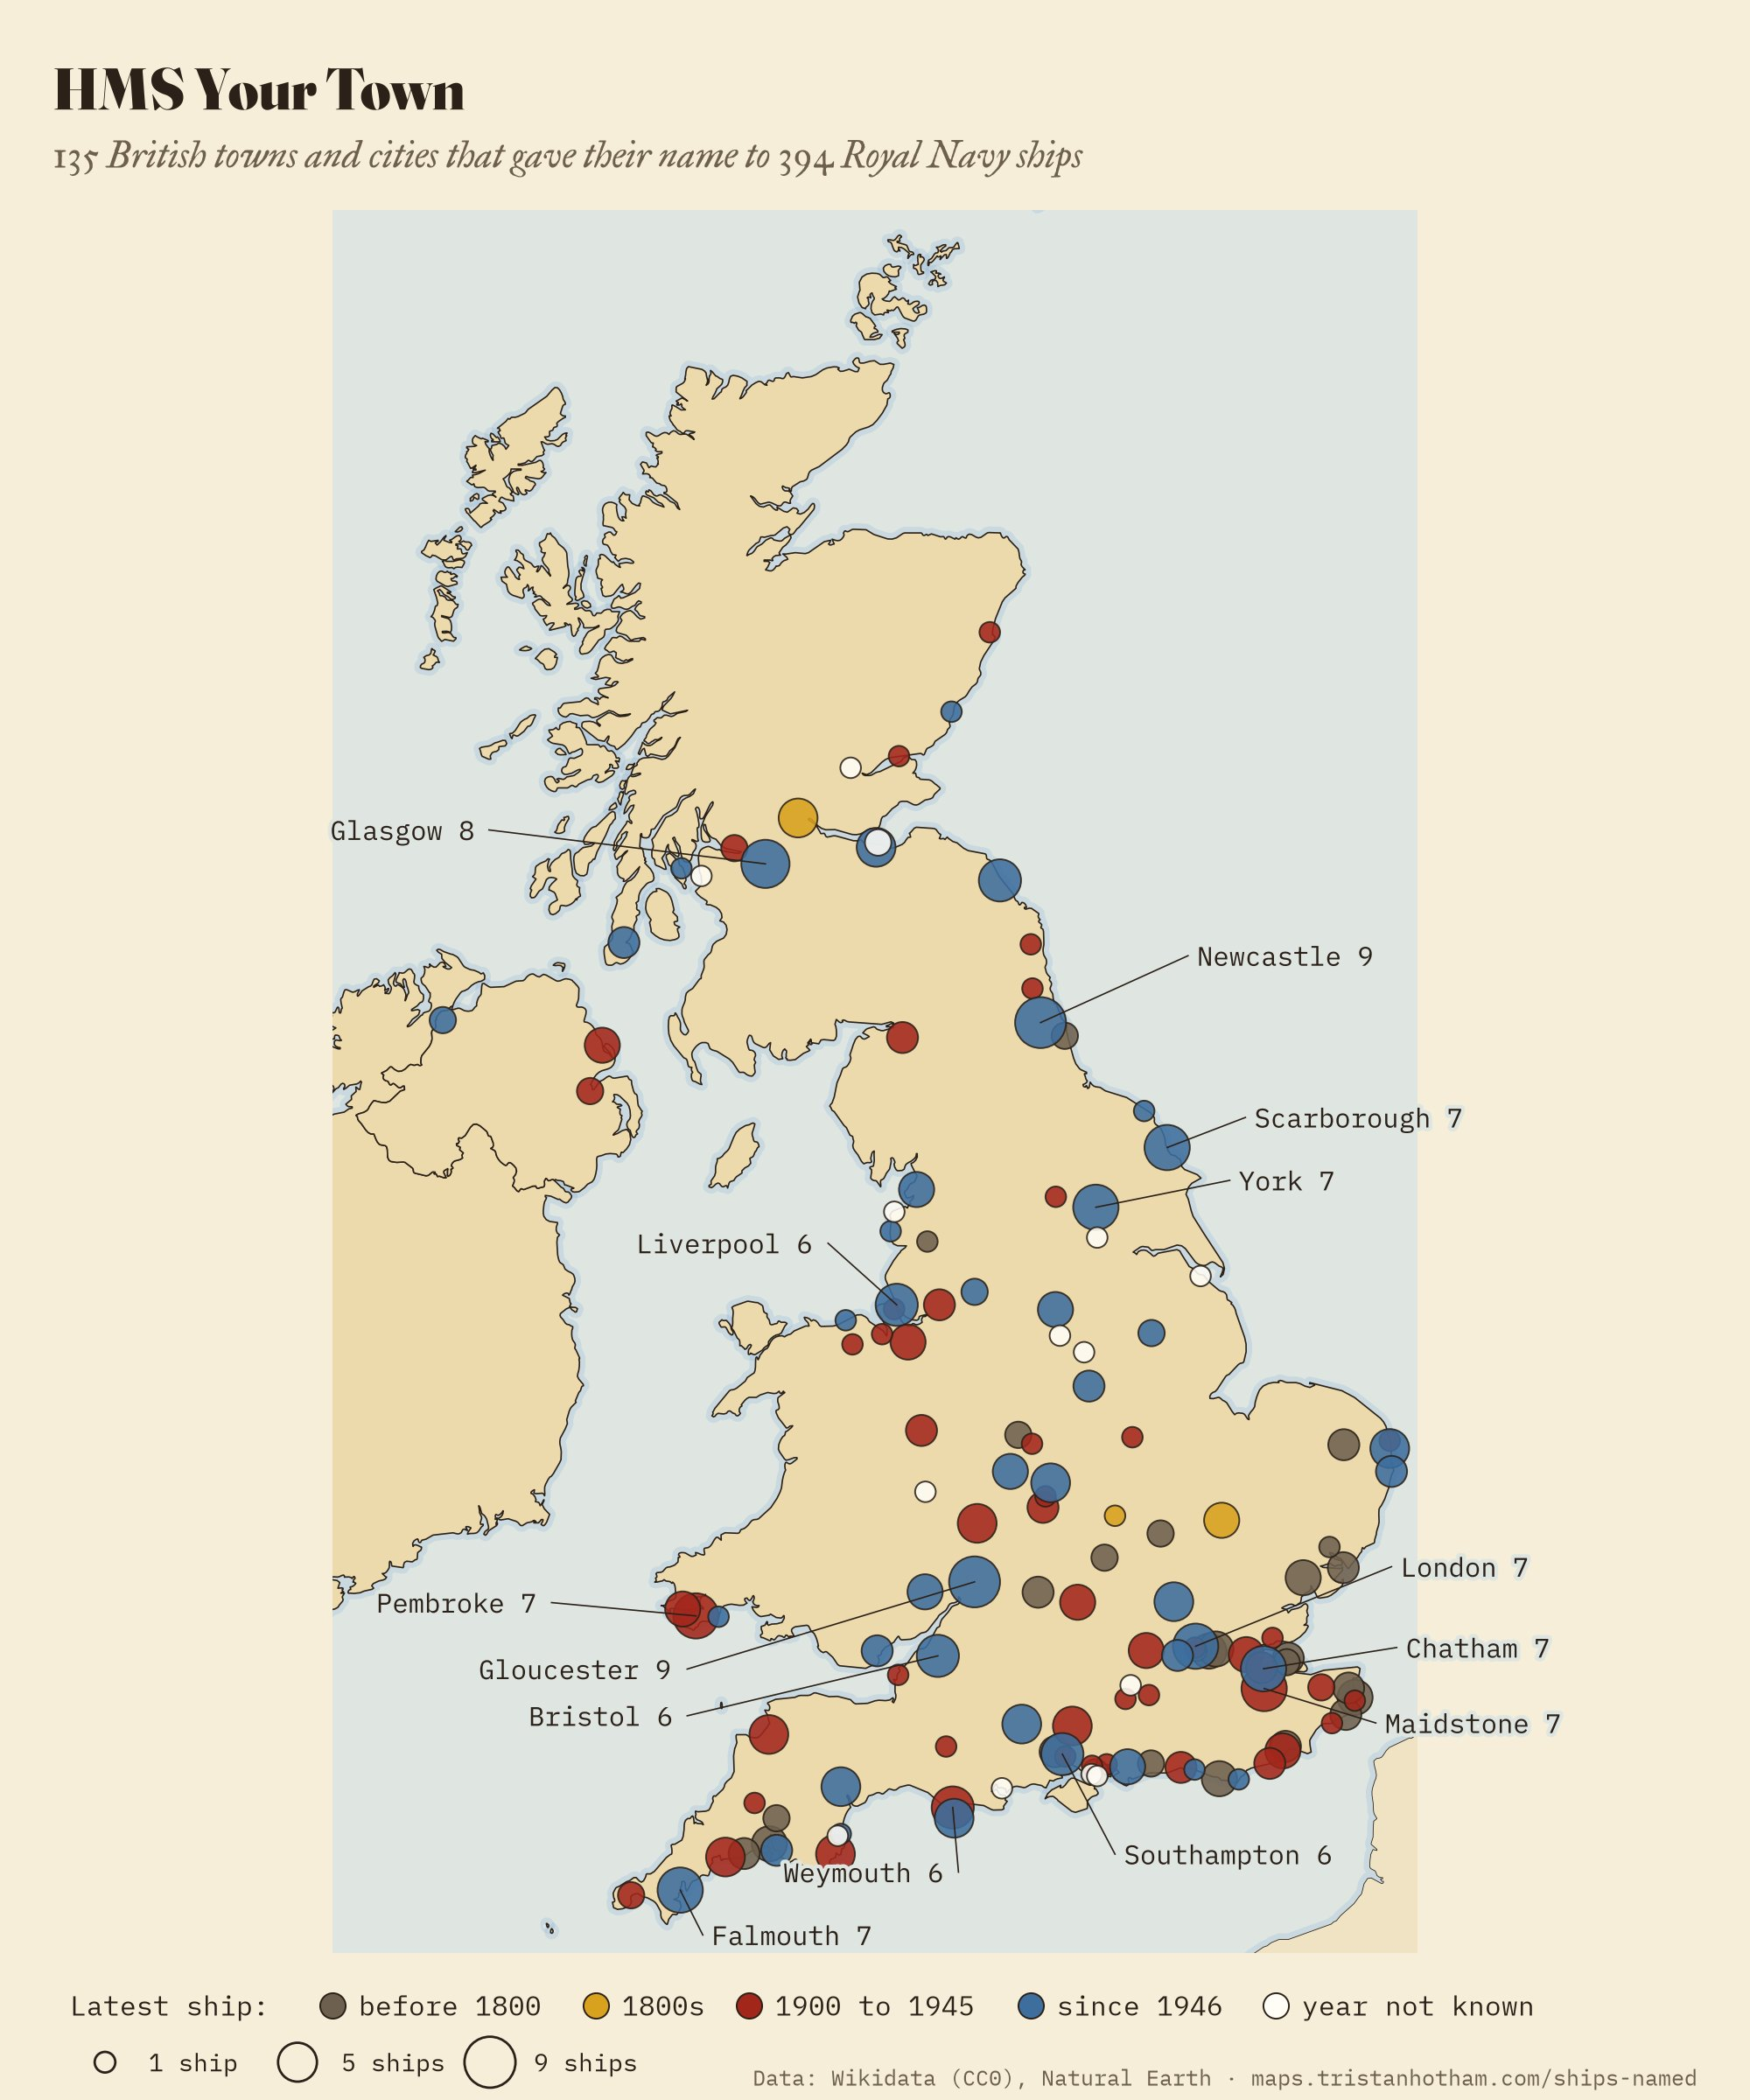
\includegraphics[width=0.82\textwidth]{f_map.jpg}
\caption{British towns and cities with a Royal Navy ship of their name, sized by the number of ships and coloured by the era of the latest.}\label{fig:map}\end{figure}
\begin{figure}[tbp]\centering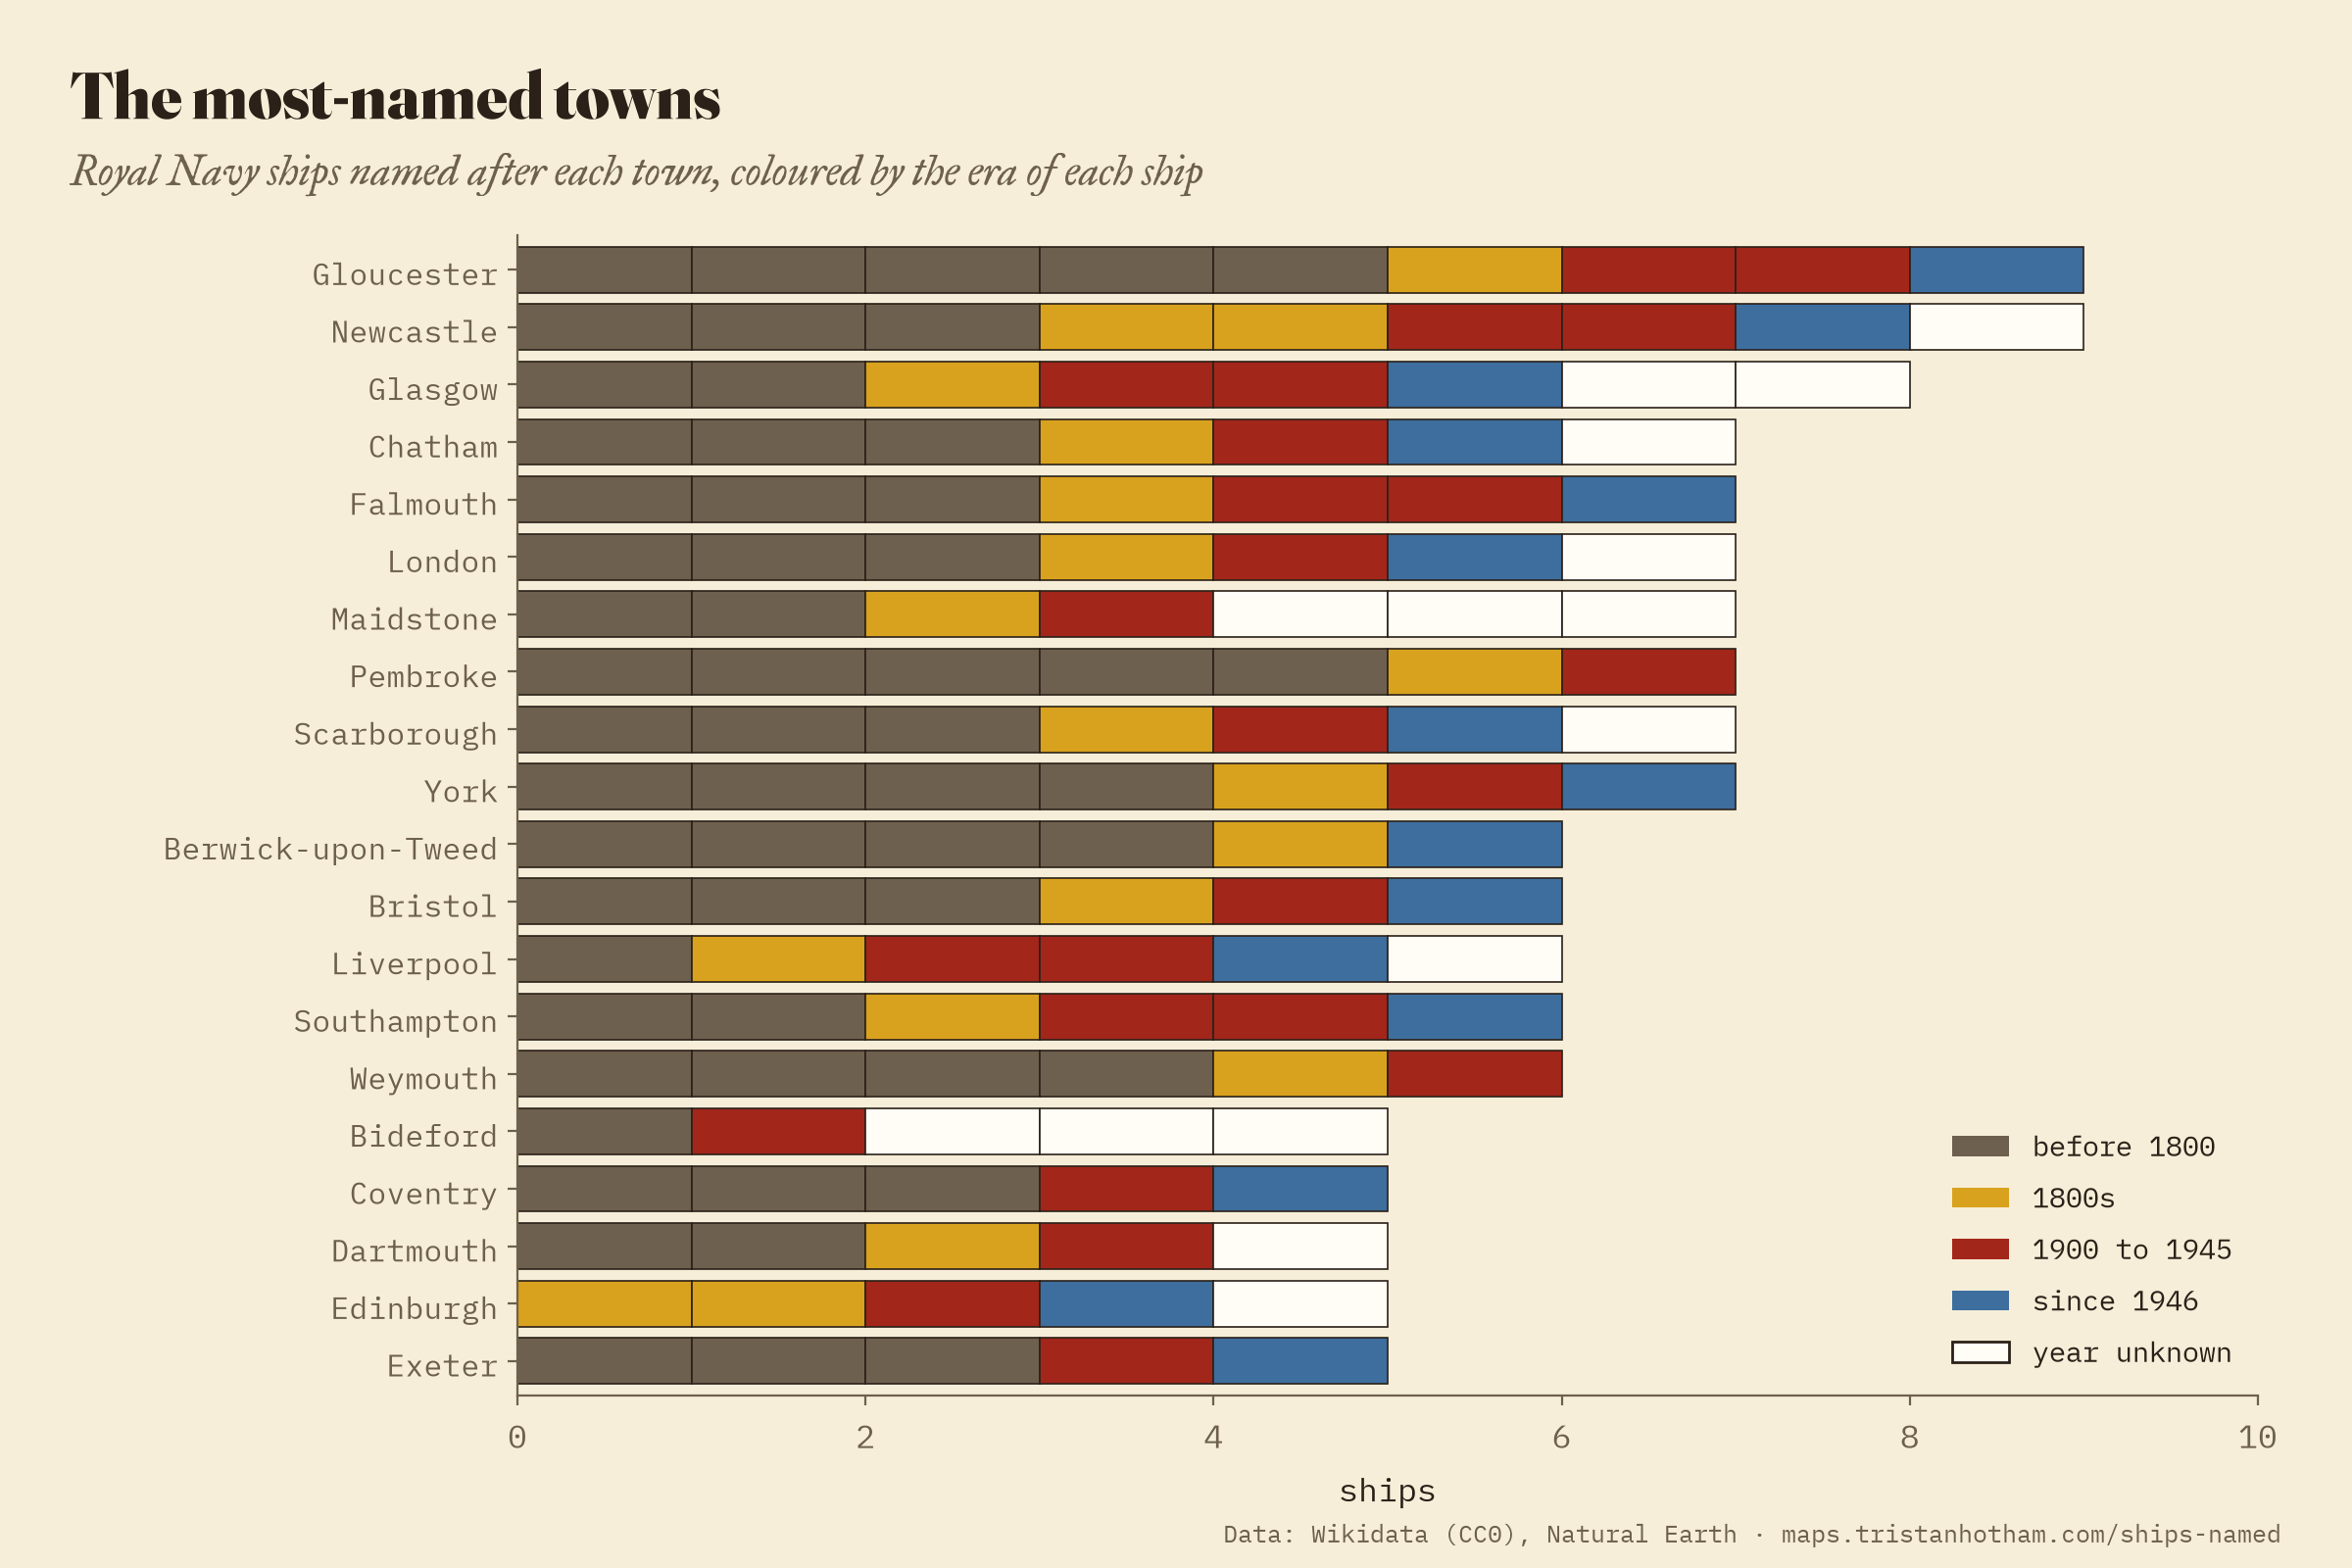
\includegraphics[width=\textwidth]{f_top.png}
\caption{The twenty towns with most ships; each block is one ship, coloured by era.}\label{fig:top}\end{figure}

\subsection{When}
Town names follow a long cycle (Figure~\ref{fig:eras}). Of the Royal Navy ships in Wikidata commissioned from 1650 to 1699, 33.3\% (65 of 195) bear a British town's name, and 30.1\% from 1700 to 1749. The share then falls to 6.4\%, 2.3\% and 1.3\% in the following half centuries, and rises again to 4.3\% in 1900 to 1949 and 22.8\% in 1950 to 1999, the years of the Castle-class corvettes (21 ships), the town-named frigates and the Type 42 destroyers named after cities (14). The early peak is partly a peak of noble titles that were also town names.

\begin{figure}[tbp]\centering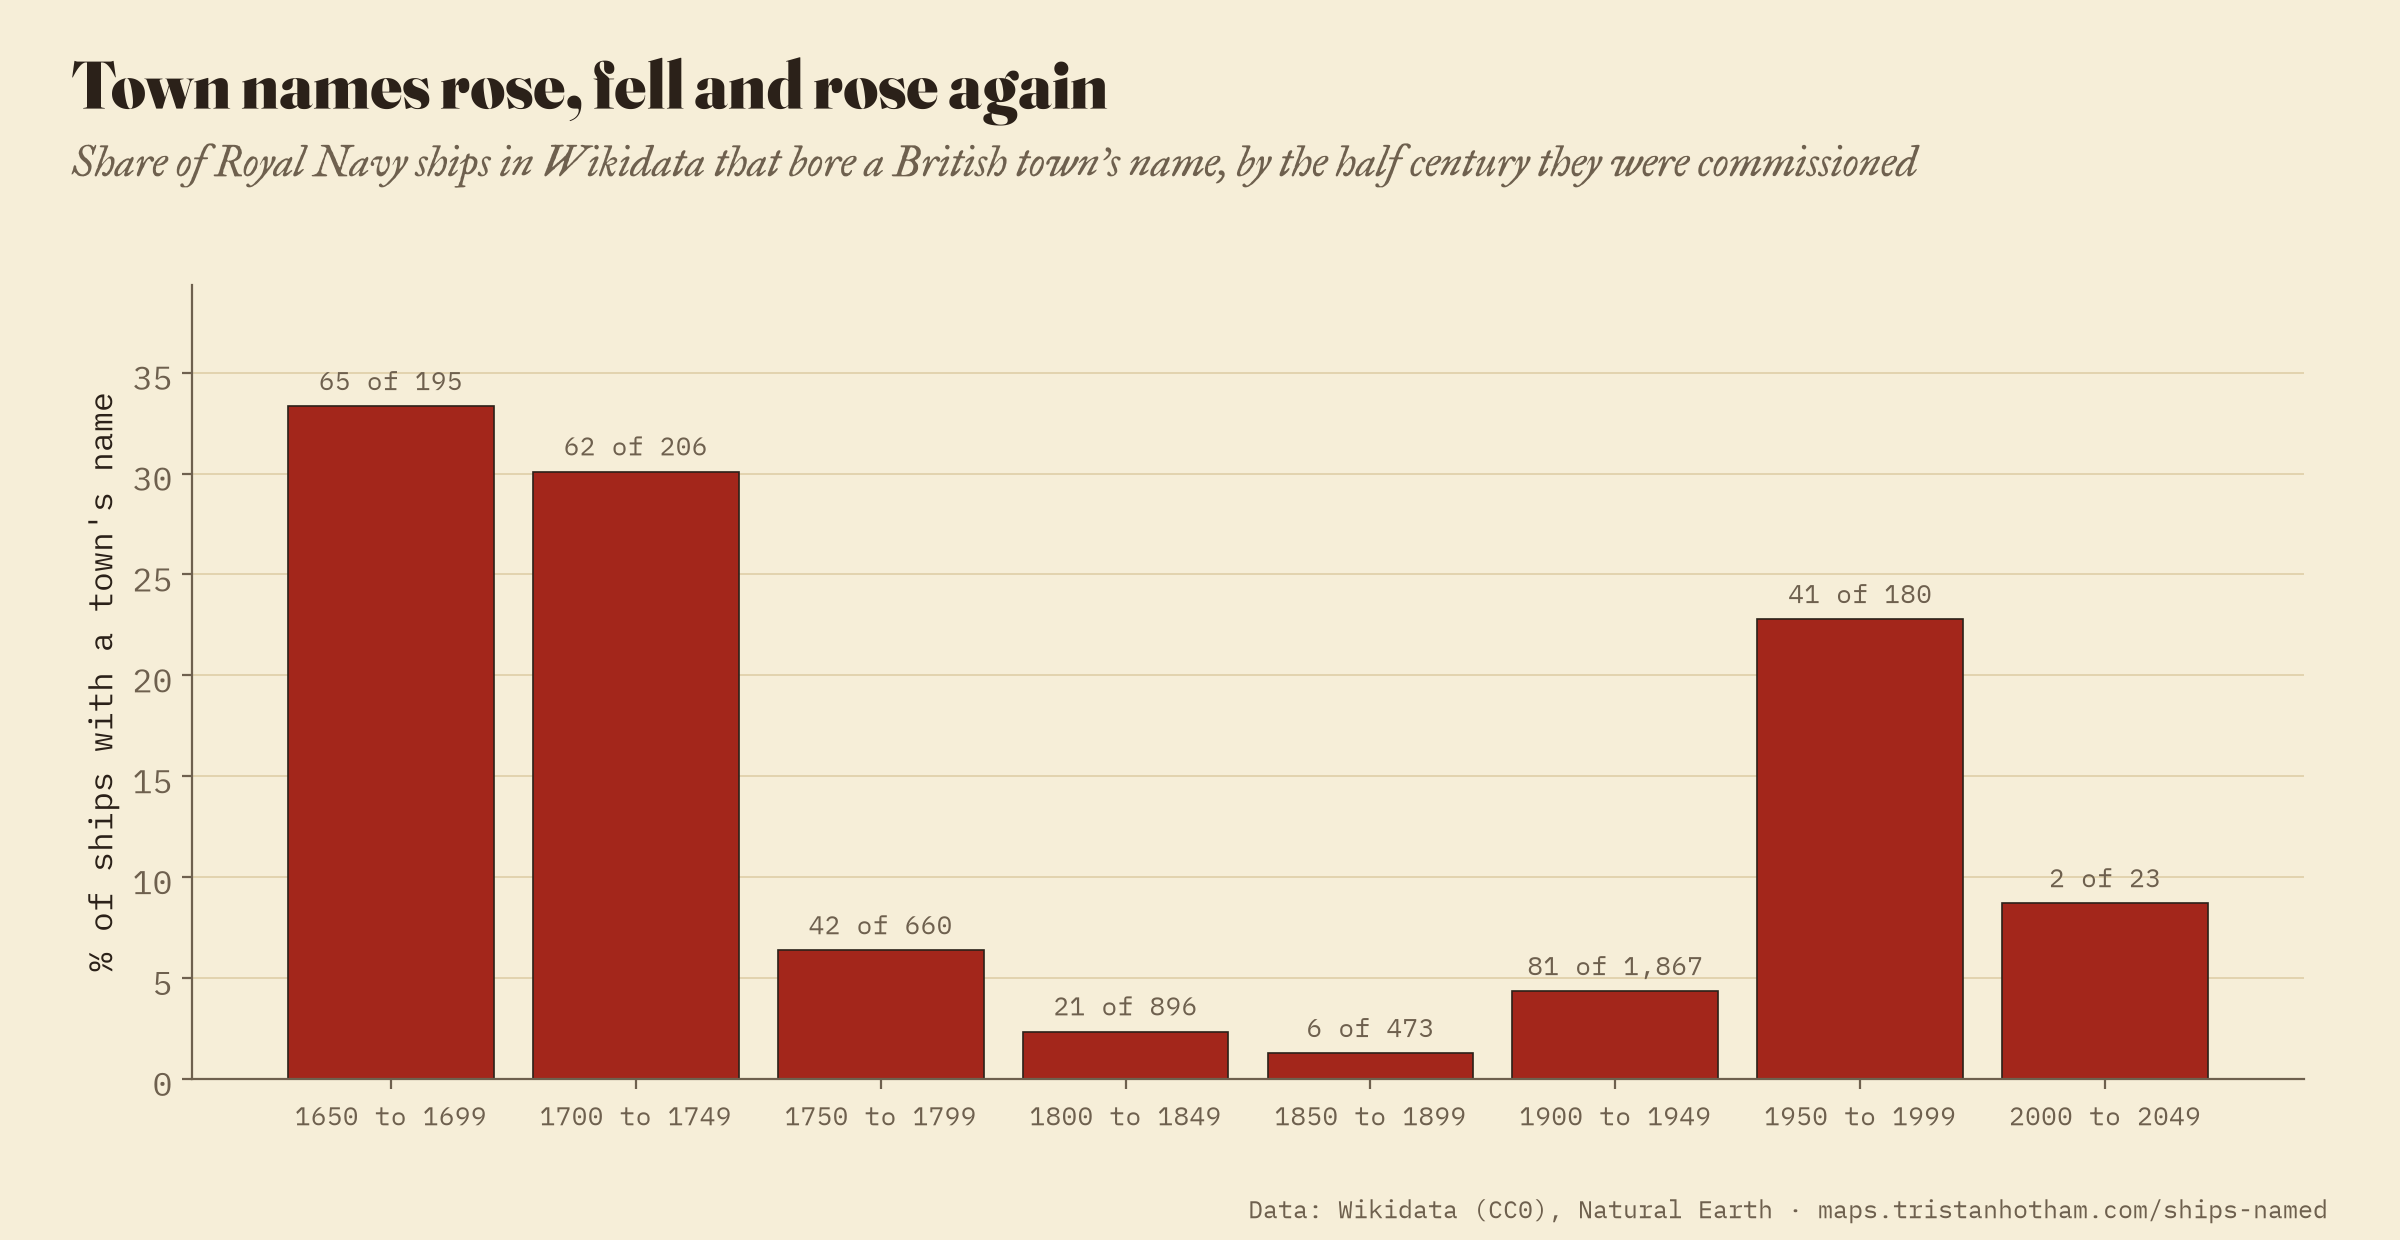
\includegraphics[width=\textwidth]{f_eras.png}
\caption{Share of Royal Navy ships with a British town's name by half century of commissioning (or the class's typical year).}\label{fig:eras}\end{figure}

\subsection{Two towns by hand}
Lancaster has 4 ships: HMS Lancaster (1694), HMS Lancaster (1797), the corvette HMS Lancaster Castle (1944) and the Type 23 frigate HMS Lancaster (1992), which like the rest of its class is named after a dukedom. The Monmouth-class armoured cruiser of 1902 is excluded as one of a class named after counties, and the Town-class destroyer of 1940 is in Wikidata only under its American name. Barrow-in-Furness, a great shipbuilding town, has none in the data.

\subsection{Fates}
Only 94 of the 394 ships (23.9\%) have any recorded end (Figure~\ref{fig:fates}): 76 only a decommissioning, 11 a loss, 2 a breaking up, and 5 are recent ships with no end recorded. The recorded losses include HMS Gloucester (sunk off Crete in 1941) and HMS Sheffield and HMS Coventry (lost in the Falklands in 1982). Wikidata simply does not hold the fate of most Royal Navy ships, and a map of fates is mostly a map of gaps.

\begin{figure}[tbp]\centering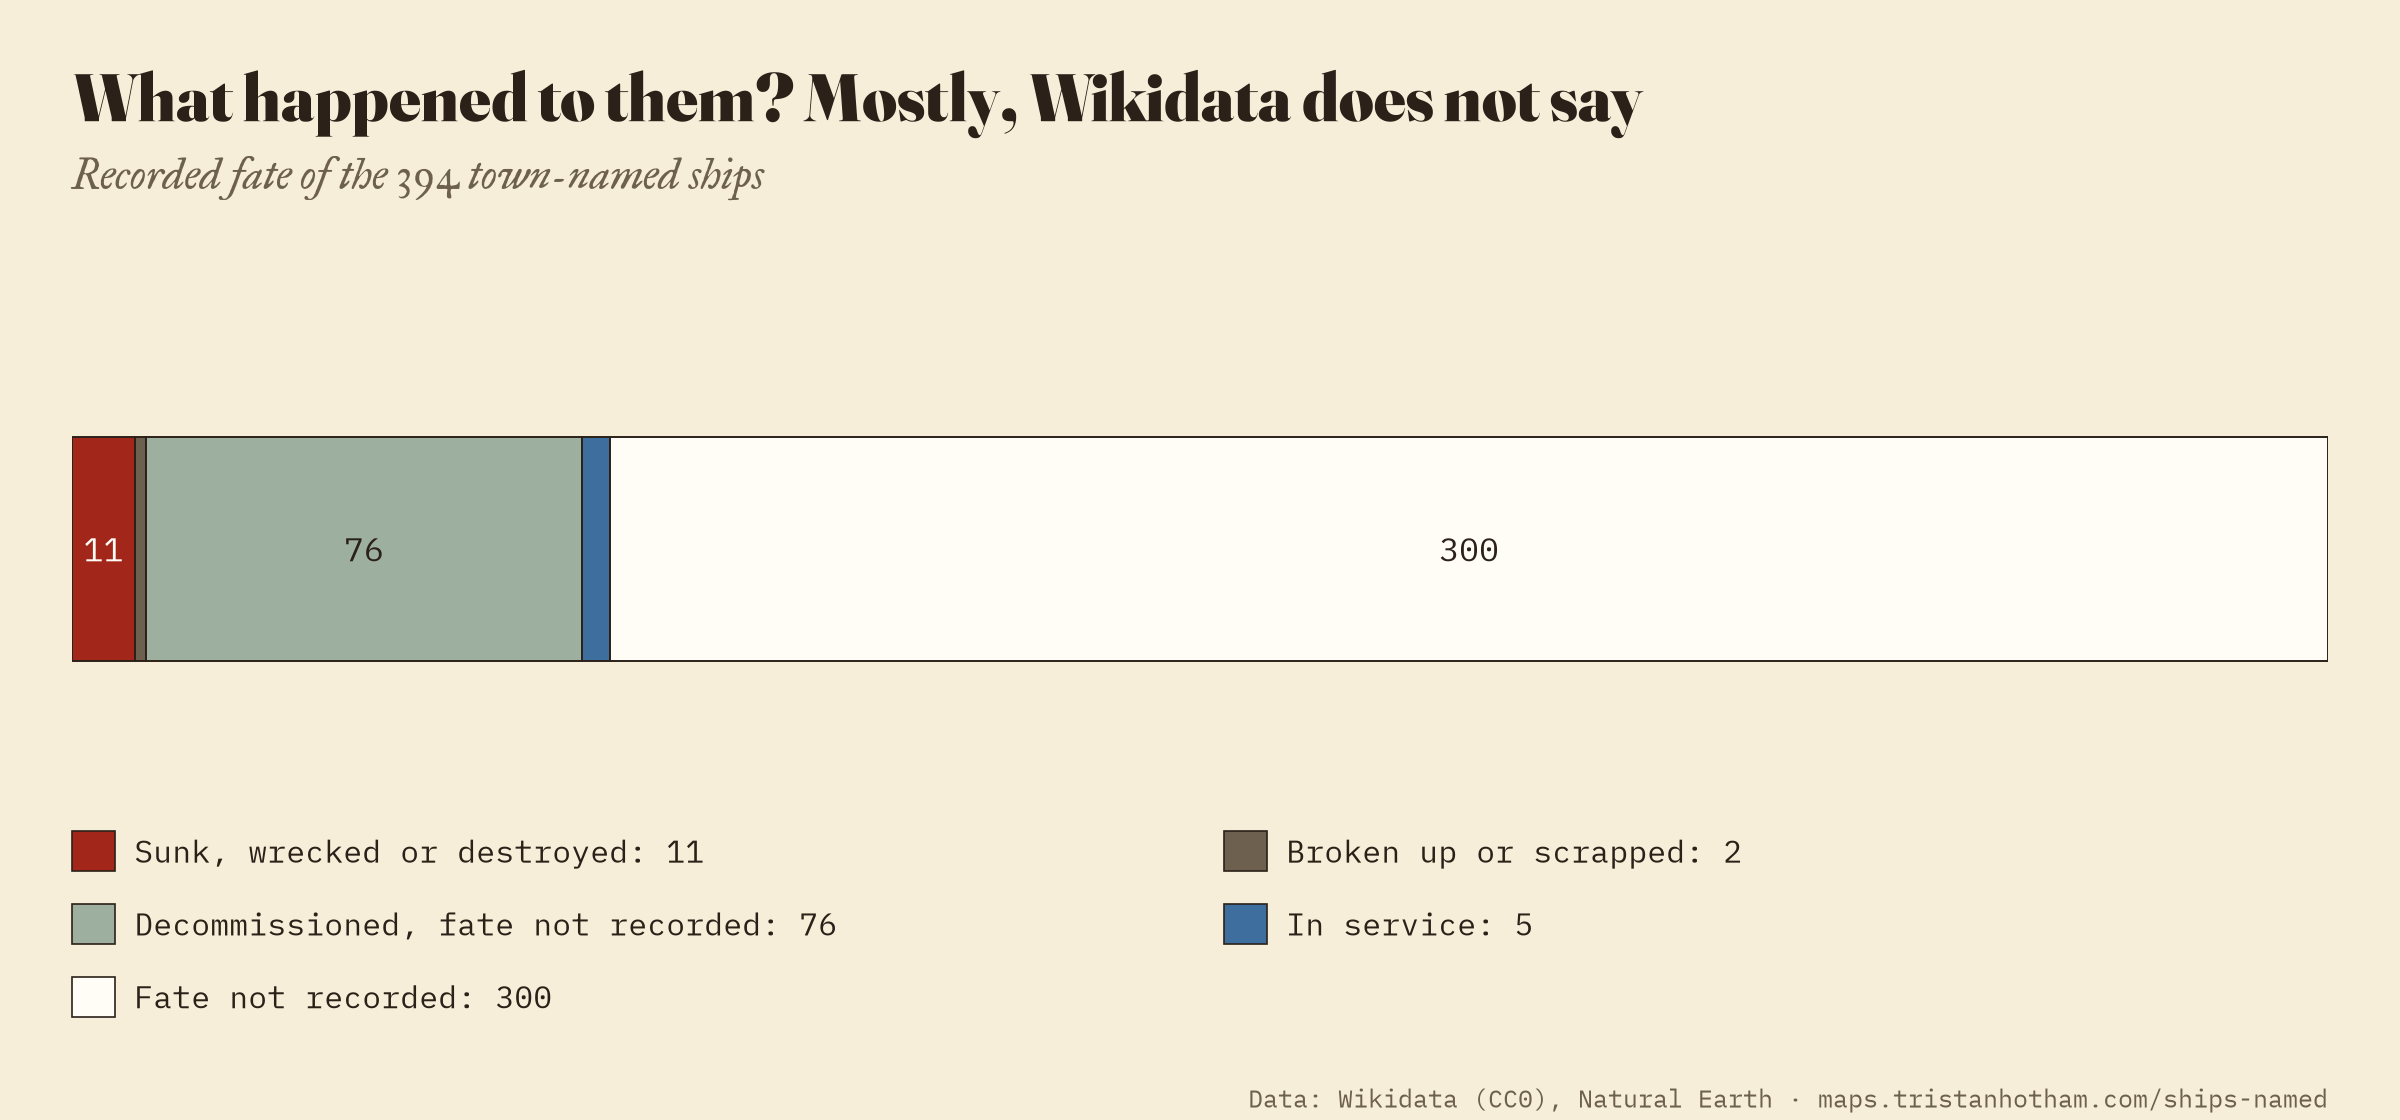
\includegraphics[width=\textwidth]{f_fates.png}
\caption{Recorded fates of the town-named ships.}\label{fig:fates}\end{figure}

\subsection{Other navies}
Among ships of all navies whose Wikidata entry names the place they honour, the United States Navy has 470, 146 of them named after American towns and cities (Figure~\ref{fig:intl}). The Royal Australian Navy also names ships mainly after its towns, while the Imperial Japanese Navy's place-named ships honour mountains, rivers and provinces, almost never towns. These counts reflect how often Wikidata records P138, which varies by navy, more than the navies' habits.

\begin{figure}[tbp]\centering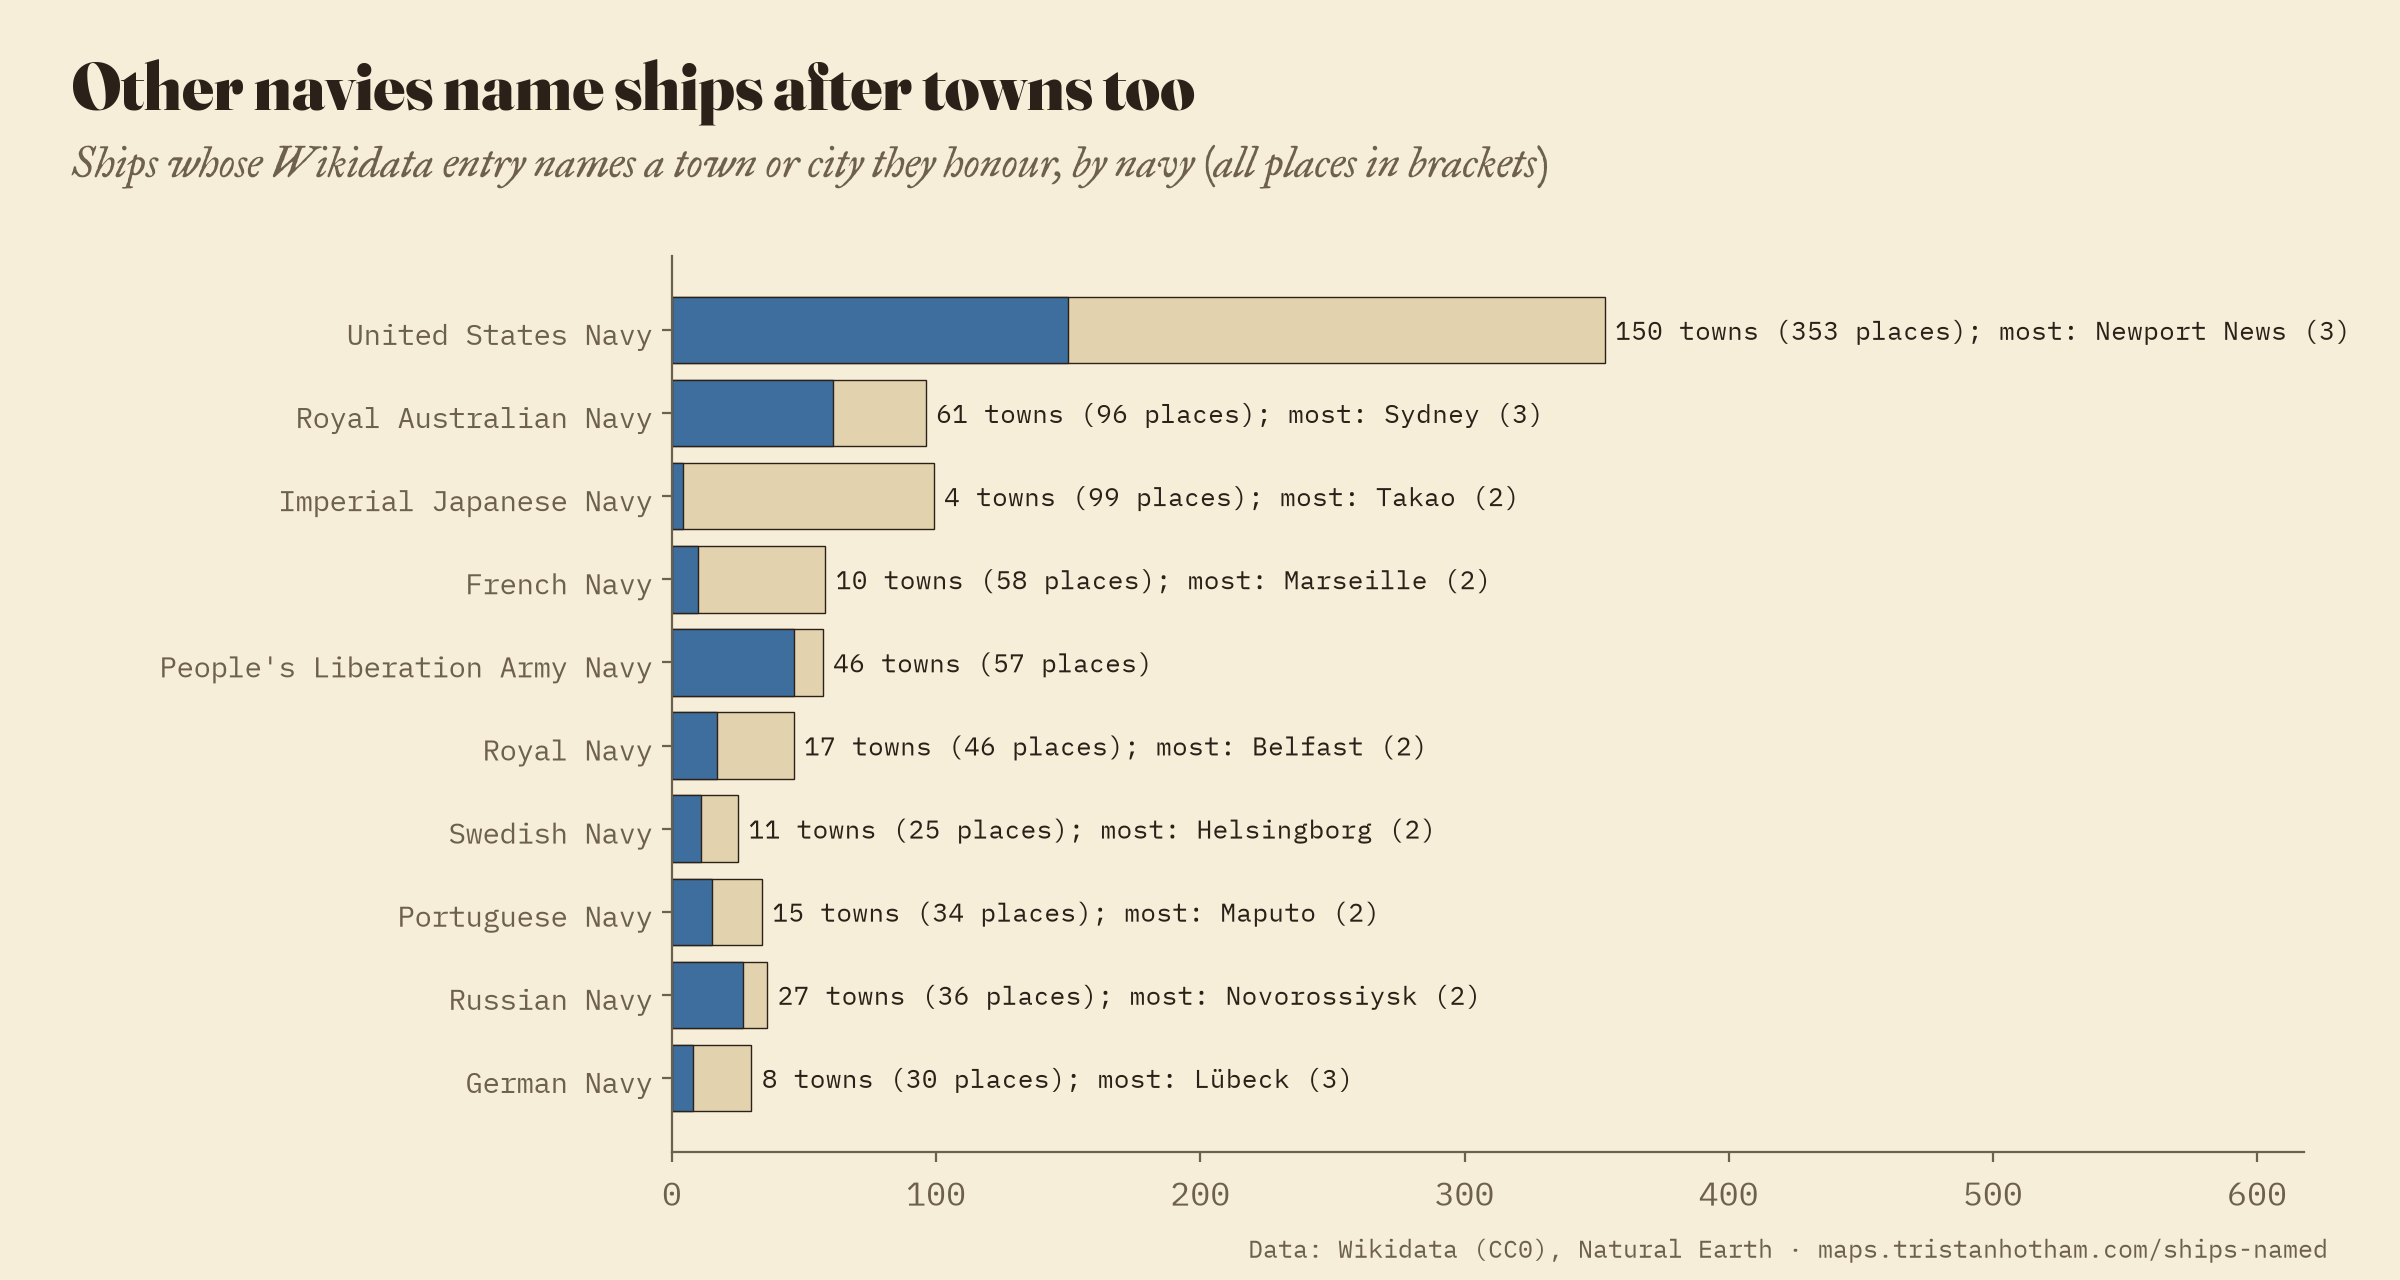
\includegraphics[width=\textwidth]{f_intl.png}
\caption{Ships named after towns and cities (blue) among ships named after any place, by navy, from Wikidata's ``named after''.}\label{fig:intl}\end{figure}

\section{Limitations}
Wikidata's list of Royal Navy ships is long but incomplete and uneven across periods. Only 261 of the 6,006 ships (4.3\%) record what they were named after, and the matched ships are 6.6\% of all of them. Whole groups can be missing: 43 of the 45 Town-class destroyers transferred from the United States in 1940, each named after a town common to both countries, are in Wikidata only under their American names. 167 matched ships (42.4\%) carry a name that is also a noble title; without them 227 ships and 93 towns remain. Matching by name is inference: a ship may honour a duke whose title is a town, or a different place of the same name, and some names in the excluded list could honour a town after all. Years are missing for some ships and approximate for others. Fates are recorded for a quarter of the ships, so nothing here measures how many town-named ships were lost. A printed register such as \citet{colledge} would fill many of these gaps.

\section{Conclusion}
A warship of the town's name is an old and widespread honour: 135 British towns in the data have had one, mostly ports and old cities, and the fashion has come and gone over three and a half centuries. What became of the ships is the part the open record cannot yet tell.

\section*{Data and code availability}
Derived data (each matched ship with its town, year and recorded fate; each town; the international table), the exclusion rules and all code are at \url{https://github.com/Tristan-Hotham/ships-named} and in the Zenodo record https://doi.org/10.5281/zenodo.24052719. Code MIT; text, figures and derived data CC BY 4.0. Source data from Wikidata (CC0).

\section*{AI statement}
I wrote the text, with drafting and editing assistance from Claude (Anthropic), which also helped prepare the analysis code. I reviewed and checked all text and results.

\begin{thebibliography}{9}
\bibitem[Colledge and Warlow(2006)]{colledge} Colledge, J. J. and Warlow, B. (2006) \textit{Ships of the Royal Navy: The Complete Record of all Fighting Ships of the Royal Navy}. Revised edition. London: Chatham Publishing.
\bibitem[Natural Earth(2026)]{naturalearth} Natural Earth (2026) Admin 0 countries, 1:10m. Public domain. \url{https://www.naturalearthdata.com/}
\bibitem[Wikidata(2026)]{wikidata} Wikidata (2026) Wikidata, the free knowledge base. CC0. \url{https://www.wikidata.org/}
\end{thebibliography}

\appendix
\section{Every town}
{\footnotesize\begin{longtable}{llrrrl}\caption{Every British town or city with a Royal Navy ship of its name in the data, by number of ships. Title: the name is also a noble title.}\\\toprule Town & Nation & Ships & First & Latest & Title\\\midrule\endfirsthead\toprule Town & Nation & Ships & First & Latest & Title\\\midrule\endhead
Gloucester & England & 9 & 1654 & 1985 & yes\\
Newcastle upon Tyne & England & 9 & 1653 & 1978 & yes\\
Glasgow & Scotland & 8 & 1741 & 1979 & \\
Chatham & England & 7 & 1691 & 1990 & \\
Falmouth & England & 7 & 1693 & 1961 & \\
London & England & 7 & 1656 & 1987 & \\
Maidstone & England & 7 & 1744 & 1937 & \\
Pembroke & Wales & 7 & 1689 & 1944 & yes\\
Scarborough & England & 7 & 1708 & 1957 & \\
York & England & 7 & 1654 & 1985 & yes\\
Berwick-upon-Tweed & England & 6 & 1689 & 1961 & \\
Bristol & England & 6 & 1653 & 1973 & yes\\
Liverpool & England & 6 & 1758 & 1982 & \\
Southampton & England & 6 & 1693 & 1981 & yes\\
Weymouth & England & 6 & 1693 & 1911 & \\
Bideford & England & 5 & 1733 & 1932 & \\
Coventry & England & 5 & 1658 & 1978 & yes\\
Dartmouth & England & 5 & 1693 & 1911 & yes\\
Edinburgh & Scotland & 5 & 1811 & 1985 & yes\\
Exeter & England & 5 & 1680 & 1980 & yes\\
Fowey & England & 5 & 1744 & 1931 & \\
Great Yarmouth & England & 5 & 1653 & 1960 & \\
Portland & England & 5 & 1653 & 2001 & yes\\
Salisbury & England & 5 & 1698 & 1958 & yes\\
St Albans & England & 5 & 1687 & 2002 & yes\\
Stirling & Scotland & 5 & 1679 & 1811 & \\
Winchester & England & 5 & 1693 & 1918 & yes\\
Worcester & England & 5 & 1698 & 1922 & yes\\
Birmingham & England & 4 & 1914 & 1976 & \\
Cambridge & England & 4 & 1666 & 1815 & yes\\
Chester & England & 4 & 1691 & 1916 & yes\\
Chichester & England & 4 & 1695 & 1958 & yes\\
Colchester & England & 4 & 1694 & 1746 & \\
Deal & England & 4 & 1708 & 1756 & \\
Greenwich & England & 4 & 1666 & 1747 & \\
Lancaster & England & 4 & 1694 & 1992 & yes\\
Larne & Northern Ireland & 4 & 1813 & 1943 & \\
Milford Haven & Wales & 4 & 1759 & 1932 & \\
Monmouth & Wales & 4 & 1667 & 1993 & yes\\
Oxford & England & 4 & 1674 & 1944 & yes\\
Saltash & England & 4 & 1745 & 1745 & \\
Seaford & England & 4 & 1733 & 1733 & \\
Sheffield & England & 4 & 1937 & 1988 & \\
Tilbury & England & 4 & 1699 & 1918 & \\
Winchelsea & England & 4 & 1733 & 1918 & yes\\
Windsor & England & 4 & 1695 & 1918 & yes\\
Woolwich & England & 4 & 1675 & 1749 & \\
Burford & England & 3 & 1679 & 1757 & yes\\
Campbeltown & Scotland & 3 & 1940 & 1989 & \\
Cardiff & Wales & 3 & 1916 & 1979 & \\
Carlisle & England & 3 & 1693 & 1918 & yes\\
Dover & England & 3 & 1654 & 1654 & \\
Harwich & England & 3 & 1674 & 1743 & \\
Hastings & England & 3 & 1694 & 1930 & \\
Looe & England & 3 & 1694 & 1741 & \\
Lowestoft & England & 3 & 1914 & 1961 & \\
Norwich & England & 3 & 1691 & 1745 & \\
Nottingham & England & 3 & 1703 & 1983 & yes\\
Orford & England & 3 & 1698 & 1916 & yes\\
Plymouth & England & 3 & 1653 & 1961 & yes\\
Redbridge & England & 3 & 1798 & 1798 & \\
Richmond & England & 3 & 1757 & 1995 & yes\\
Rochester & England & 3 & 1693 & 1932 & yes\\
Rye & England & 3 & 1708 & 1733 & \\
Sandwich & England & 3 & 1679 & 1759 & yes\\
Sheerness & England & 3 & 1741 & 1741 & \\
Shoreham-by-Sea & England & 3 & 1708 & 1932 & \\
Shrewsbury & England & 3 & 1695 & 1944 & yes\\
Warwick & England & 3 & 1696 & 1918 & yes\\
Arundel & England & 2 & 1751 & 1751 & yes\\
Bedford & England & 2 & 1698 & 1775 & yes\\
Belfast & Northern Ireland & 2 & 1939 & 1939 & \\
Buckingham & England & 2 & 1731 & 1751 & yes\\
Canterbury & England & 2 & 1693 & 1915 & \\
Derry & Northern Ireland & 2 & 1961 & 1961 & \\
Dumbarton & Scotland & 2 & 1944 & 1944 & \\
Leith & Scotland & 2 &  &  & \\
Lichfield & England & 2 & 1695 & 1746 & \\
Lincoln & England & 2 & 1695 & 1960 & yes\\
Manchester & England & 2 & 1938 & 1982 & \\
Penzance & England & 2 & 1931 & 1931 & \\
Portsmouth & England & 2 & 1650 & 1650 & yes\\
Queenborough & England & 2 & 1751 & 1751 & \\
Sunderland & England & 2 & 1694 & 1724 & yes\\
Tavistock & England & 2 & 1745 & 1747 & yes\\
Aberdeen & Scotland & 1 & 1936 & 1936 & \\
Alnwick & England & 1 & 1944 & 1944 & \\
Birkenhead & England & 1 & 1915 & 1915 & \\
Blackpool & England & 1 & 1958 & 1958 & \\
Brighton & England & 1 & 1961 & 1961 & \\
Caister-on-Sea & England & 1 & 1944 & 1944 & \\
Chesterfield & England & 1 &  &  & yes\\
Denbigh & Wales & 1 & 1944 & 1944 & \\
Dundee & Scotland & 1 & 1933 & 1933 & \\
Eastbourne & England & 1 & 1958 & 1958 & \\
Farnborough & England & 1 &  &  & \\
Farnham & England & 1 & 1945 & 1945 & \\
Fleetwood & England & 1 &  &  & \\
Flint & Wales & 1 & 1944 & 1944 & \\
Folkestone & England & 1 & 1930 & 1930 & \\
Gosport & England & 1 &  &  & \\
Grimsby & England & 1 &  &  & \\
Guildford & England & 1 & 1944 & 1944 & \\
Hadleigh & England & 1 & 1943 & 1943 & \\
Havant & England & 1 & 1939 & 1939 & \\
Ipswich & England & 1 & 1694 & 1694 & \\
Kenilworth & England & 1 & 1943 & 1943 & \\
Kennington & England & 1 & 1733 & 1733 & \\
Knaresborough & England & 1 & 1944 & 1944 & \\
Largs & Scotland & 1 &  &  & \\
Launceston & England & 1 & 1944 & 1944 & \\
Ludlow & England & 1 &  &  & yes\\
Mansfield & England & 1 &  &  & \\
Montrose & Scotland & 1 & 1994 & 1994 & yes\\
Morpeth & England & 1 & 1944 & 1944 & \\
Northampton & England & 1 & 1876 & 1876 & yes\\
Oakham & England & 1 & 1944 & 1944 & \\
Perth & Scotland & 1 &  &  & yes\\
Poole & England & 1 &  &  & \\
Portchester & England & 1 & 1944 & 1944 & \\
Preston & England & 1 & 1757 & 1757 & \\
Rhyl & Wales & 1 & 1960 & 1960 & \\
Rothesay & Scotland & 1 & 1960 & 1960 & \\
Selby & England & 1 &  &  & \\
Sherborne & England & 1 & 1944 & 1944 & \\
Southsea & England & 1 &  &  & \\
Tamworth & England & 1 & 1944 & 1944 & \\
Tenby & Wales & 1 & 1957 & 1957 & \\
Torbay & England & 1 &  &  & \\
Torquay & England & 1 & 1956 & 1956 & \\
Walmer & England & 1 & 1944 & 1944 & \\
Westminster & England & 1 & 1918 & 1918 & \\
Weston-super-Mare & England & 1 & 1932 & 1932 & \\
Whitby & England & 1 & 1956 & 1956 & \\
Woolston & England & 1 & 1918 & 1918 & \\
\bottomrule\end{longtable}}
\end{document}
